This chapter describes the implementation details of the JS-QL framework and language, as presented in chapter \ref{ch:JSQL}. The implementation of JS-QL is publicly available\footnote{https://github.com/voluminat0/Jipda-Security} and can freely be used to test source code for characteristics and vulnerabilities.


\section{Architecture}
The architecture of the implementation separates each component in a different module, providing the possibility to replace these modules by alternative implementations. In this section we discuss what each component represents.

\subsection*{Datastructures}
The \texttt{DataStructures} module defines all datastructures used in JS-QL. These include all kinds of tuples used for our matching algorithm, but also the alternative representations of edges and nodes to transform the abstract state graph to a compatible graph for the matching engine.

\subsection*{AbstractQuery}
The \texttt{AbstractQuery} module defines the core of the matching engine. It contains all operations on substitution sets: Matching, merging, defining extra properties, filters and lookups. The module provides an interface to the actual query algorithms \texttt{ExistentialQuery} and \texttt{UniversalQuery}, which perform the actual query matching processes.

\subsection*{Automaton}
The \texttt{Automaton} module defines the uniform representation of finite state machines (also known as finite automatons). It abstracts away whether the automaton is a deterministic or non-deterministic automaton, and provides information about the accepting states and starting state of these automatons.

\subsubsection*{ThompsonConstruction}
The \texttt{ThompsonConstruction} module defines an algorithm to convert a regular expression to a NFA (non-deterministic finite automaton). It parses the regular path expression and adds zero or more states to the newly created automaton for each step in the parsing process.
\subsubsection*{SubsetConstruction}
The \texttt{ThompsonConstruction} module defines an algorithm to convert a NFA to a DFA (deterministic finite automaton). What this means is that it eliminates all $\epsilon$-transitions, which are transitions that can occur without reading an input symbol. The resulting automaton is used for both query algorithms.

\subsection*{JipdaInfo}
The \texttt{JipdaInfo} module transforms state information to a more readable format for users. This transformation is necessary to have enforce consistency in states representing an AST node. The transformed states are the actual states that are queried instead of the original JIPDA states.

\subsection*{JSQL}
The \texttt{JSQL} module defines the internals of the JS-QL query language. It is implemented as an embedded DSL in JavaScript and allows users to define application-specific predicates and policies. The module is made available for the user through a fluent interface, increasing the readability of the language.

\subsection*{SecurityAnalysis}
The \texttt{SecurityAnalysis} module glues every component together in the framework. The initialization and transformation of the abstract state graph, execution of queries and processing query results are all invoked by this module.

\section{The user interface}
The JIPDA analysis comes packed with an interface which enables the user to inspect the abstract state graph. This state graph is generated when the user provides an input program and a lattice to perform the abstract interpretation. For our framework we augmented this user interface in several ways described in this section. Figure \ref{fig:UI} shows the user interface, illustrating what we will discuss in the next sections.

\begin{figure}[h]
    \centering
      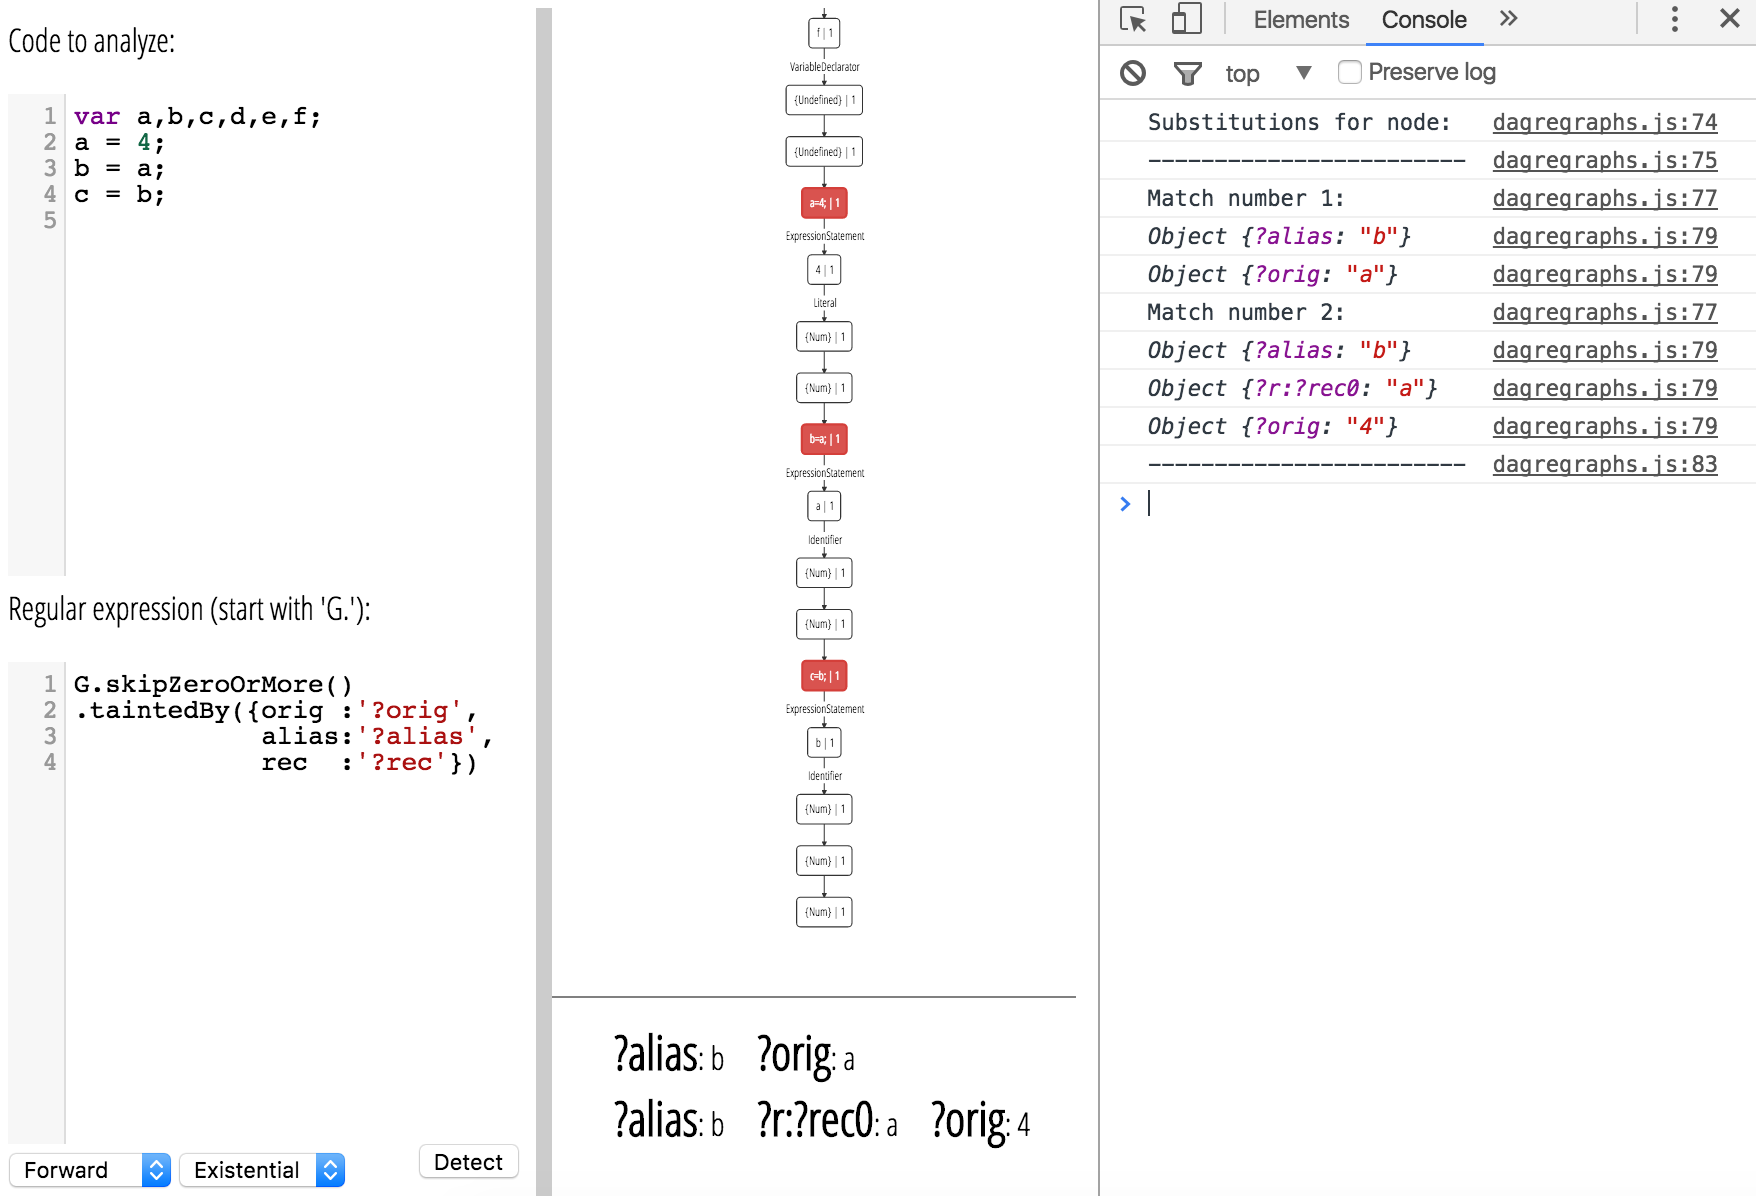
\includegraphics[width=1\textwidth]{images/UI} 
      \caption{The JS-QL framework user interface}
    \label{fig:UI}
\end{figure}

\subsection*{Query interpretation}

We decided to allow the user to specify queries in the user interface itself. In this way we avoid to switch between different screens and/or files to run just one query. The user interface contains a third-party JavaScript plugin which enables syntax highlighting. We use this plugin as input textboxes for a query and the input program. Along with entering the needed information, a user can decide the kind of query that needs to be executed. This can be done by selecting the direction together with type of query (existential or universal). When hitting the 'detect' button, internally a new \texttt{Query} object is made with the provided query string. Query objects contain three fields: The query direction, its type and a \texttt{JSQL} object, representing the instantiated query. Although being unsafe, the query string is converted to a JSQL object by \texttt{eval}uating it. For the sake of this dissertation, the safety of the application isn't relevant for its functionality.

\subsection*{The abstract state graph}

JIPDA already provided the functionality to display the abstract state graph in the user interface. In order to show results, this representation of the graph needed to be modified so that it became optimal for the user to reason about query results. We changed the following:
\begin{enumerate}
\item \textit{Edge labels}: The JIPDA state graph already contained edge labels, but the information they contained was irrelevant for our approach. As our approach uses edge labels to match states, we had to shift information from nodes to edges. All evaluation states's outgoing edges are also augmented with a visible edge label representing the type of AST node it contains, to make it easier for the user to see what he has to specify in his queries.
\item \textit{State colours}: The default colours of all JIPDA states have been stripped from the graph. This was done to increase the contrast with marked states (i.e. states indicating a match of the query). When the matching engine produced all results, these results have to be transferred to the corresponding states of the state graph. A 'marker' property was added to each matched state, containing the match information as well as a CSS class to highlight them in the otherwise colourless graph. This CSS class can be customised by the user.
\end{enumerate}

\subsection*{Results inspection}

Each query result is a set of substitutions, mapping variables (denoted by a starting \texttt{?}) to their corresponding values in the state graph. Every matching state is marked with its substitution set(s). These results can then be further explored through the results section under the state graph or in the browser's built-in console, which allows to inspect results in even greater detail.


\section{The query language}
The JS-QL query language is implemented as an embedded DSL with JavaScript as its host language. We motivated the use of a DSL in chapter \ref{ch:overview} and explored the JS-QL syntax and semantics in chapter \ref{ch:JSQL}. This section describes how the DSL is implemented and how we incorporated several DSL implementation techniques.

%deferred evaluation
%recursion
%tmp en rec var
%regexpart
%cond
%prop

\section{The matching engine}

%input en output uitleggen

%paper uitleggen en referencen